\documentclass[12pt]{article}

% Packages
\usepackage{geometry} % Adjust page margins
\usepackage{polski}
\usepackage{setspace} % Adjust line spacing
\usepackage{titlesec} % Customize section titles
\usepackage{lipsum} % For placeholder text
\usepackage{graphicx}
\usepackage{subcaption}
\usepackage{float}

% Page margins
\geometry{margin=1in}

% Line spacing
\onehalfspacing

% Section title formatting
\titleformat{\section}{\normalfont\Large\bfseries}{\thesection}{1em}{}
\titleformat{\subsection}{\normalfont\large\bfseries}{\thesubsection}{1em}{}
\titleformat{\subsubsection}{\normalfont\normalsize\bfseries}{\thesubsubsection}{1em}{}

% Title
\title{Model Isinga. Sprawozdanie z projektu.}
\author{Emil Olszewski, 268789}
\date{Czerwiec 2023}

\begin{document}

\maketitle

\section{Informacje wstępne}


Narzędzia użyte do wykonania projektu:


\begin{itemize}
\item Język: Julia 1.9.0
\item Biblioteki: 
\begin{itemize}
\item Statistics 1.9.0
\item Plots 1.38.12
\item JLD2 0.4.31
\end{itemize}
\item Generator liczb pseudolosowych: Xoshiro256++
\item Rysunki: Biblioteka "Plots"
\item Wsparcie sztucznej inteligencji: brak
\end{itemize}



\section{Sprawozdanie}

\subsection{Konfiguracje po 100 MCS}

W tej części zadania przeprowadzono symulacje modelu Isinga dla siatek kwadratowych o wymiarach $10$x$10$ oraz $80$x$80$ o losowej konfiguracji początkowej ($P(S_{ij} = 1) = P(S_{ij} = -1) = 0.5$) w temperaturach $T=1,\,T=2,26,\,T=4$.
\newpage
 
\begin{figure}[H]
  \centering

  \begin{subfigure}[b]{0.3\linewidth}
    \centering
    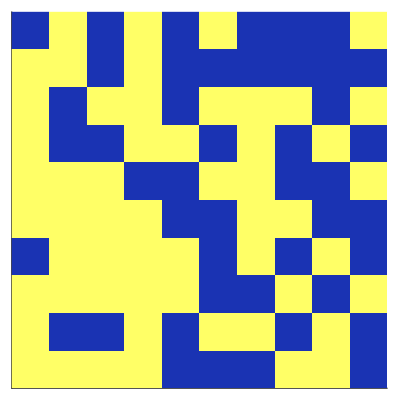
\includegraphics[width=100px, height=100px]{../data/snaps/snap10_temp1.0_moment1.png}
    \caption{MCS=0}
    \label{fig:image1}
  \end{subfigure}
  \hfill
  \begin{subfigure}[b]{0.3\linewidth}
    \centering
    
\includegraphics[width=100px, height=100px]{../data/snaps/snap10_temp1.0_moment50.png}
    \caption{MCS=50}
    \label{fig:image2}
  \end{subfigure}
  \hfill
  \begin{subfigure}[b]{0.3\linewidth}
    \centering
    
\includegraphics[width=100px, height=100px]{../data/snaps/snap10_temp1.0_moment100.png}
    \caption{MCS=100}
    \label{fig:image3}
  \end{subfigure}

  \caption{Siatka $10$x$10$, $T=1$}
  \label{fig:series}
\end{figure}

\begin{figure}[H]
  \centering

  \begin{subfigure}[b]{0.3\linewidth}
    \centering
    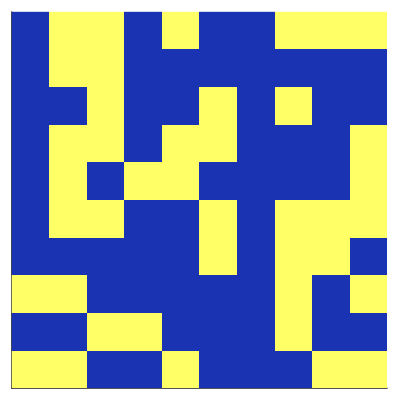
\includegraphics[width=100px, height=100px]{../data/snaps/snap10_temp2.26_moment1.png}
    \caption{MCS=0}
    \label{fig:image1}
  \end{subfigure}
  \hfill
  \begin{subfigure}[b]{0.3\linewidth}
    \centering
    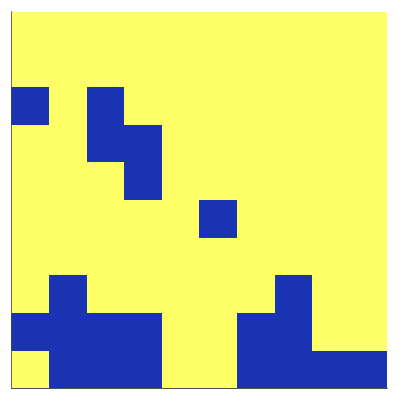
\includegraphics[width=100px, height=100px]{../data/snaps/snap10_temp2.26_moment50.png}
    \caption{MCS=50}
    \label{fig:image2}
  \end{subfigure}
  \hfill
  \begin{subfigure}[b]{0.3\linewidth}
    \centering
    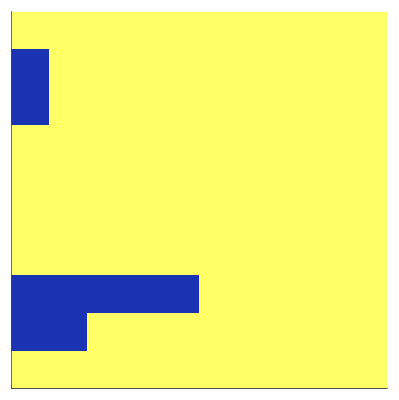
\includegraphics[width=100px, height=100px]{../data/snaps/snap10_temp2.26_moment100.png}
    \caption{MCS=100}
    \label{fig:image3}
  \end{subfigure}

  \caption{Siatka $10$x$10$, $T=2.26$}
  \label{fig:series}
\end{figure}

\begin{figure}[H]
  \centering

  \begin{subfigure}[b]{0.3\linewidth}
    \centering
    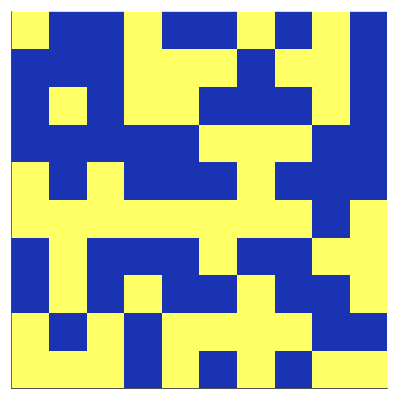
\includegraphics[width=100px, height=100px]{../data/snaps/snap10_temp4.0_moment1.png}
    \caption{MCS=0}
    \label{fig:image1}
  \end{subfigure}
  \hfill
  \begin{subfigure}[b]{0.3\linewidth}
    \centering
    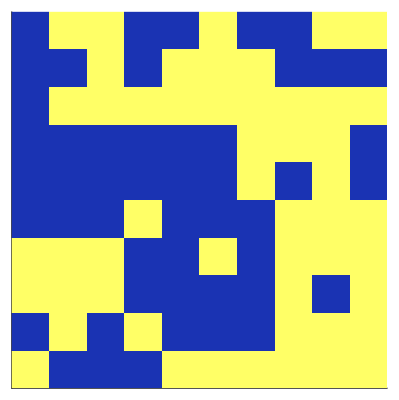
\includegraphics[width=100px, height=100px]{../data/snaps/snap10_temp4.0_moment50.png}
    \caption{MCS=50}
    \label{fig:image2}
  \end{subfigure}
  \hfill
  \begin{subfigure}[b]{0.3\linewidth}
    \centering
    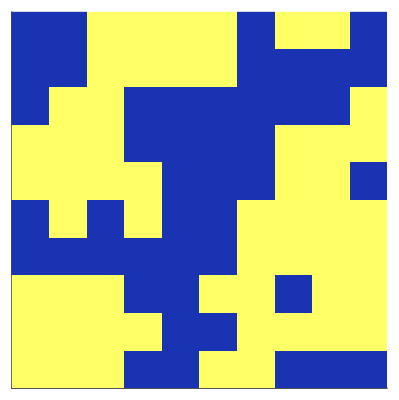
\includegraphics[width=100px, height=100px]{../data/snaps/snap10_temp4.0_moment100.png}
    \caption{MCS=100}
    \label{fig:image3}
  \end{subfigure}

  \caption{Siatka $10$x$10$, $T=4$}
  \label{fig:series}
\end{figure}

\begin{figure}[H]
  \centering

  \begin{subfigure}[b]{0.3\linewidth}
    \centering
    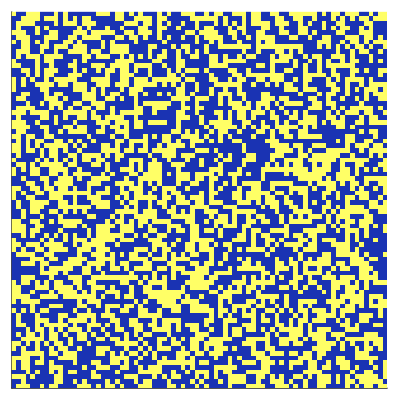
\includegraphics[width=100px, height=100px]{../data/snaps/snap80_temp1.0_moment1.png}
    \caption{MCS=0}
    \label{fig:image1}
  \end{subfigure}
  \hfill
  \begin{subfigure}[b]{0.3\linewidth}
    \centering
    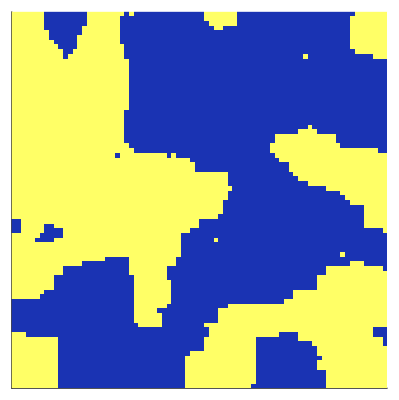
\includegraphics[width=100px, height=100px]{../data/snaps/snap80_temp1.0_moment50.png}
    \caption{MCS=50}
    \label{fig:image2}
  \end{subfigure}
  \hfill
  \begin{subfigure}[b]{0.3\linewidth}
    \centering
    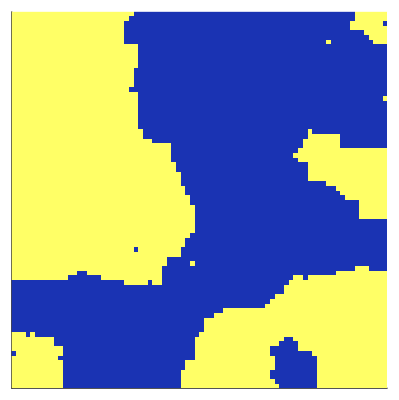
\includegraphics[width=100px, height=100px]{../data/snaps/snap80_temp1.0_moment100.png}
    \caption{MCS=100}
    \label{fig:image3}
  \end{subfigure}

  \caption{Siatka $80$x$80$, $T=1$}
  \label{fig:series}
\end{figure}

\begin{figure}[H]
  \centering

  \begin{subfigure}[b]{0.3\linewidth}
    \centering
    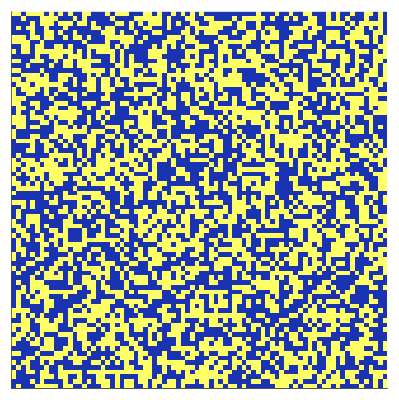
\includegraphics[width=100px, height=100px]{../data/snaps/snap80_temp2.26_moment1.png}
    \caption{MCS=0}
    \label{fig:image1}
  \end{subfigure}
  \hfill
  \begin{subfigure}[b]{0.3\linewidth}
    \centering
    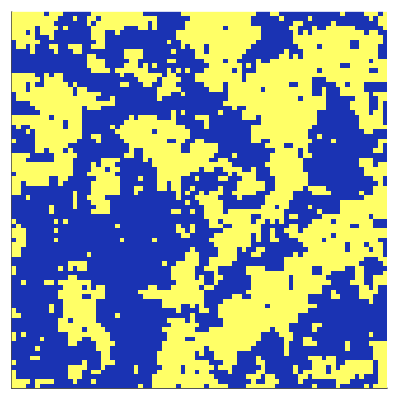
\includegraphics[width=100px, height=100px]{../data/snaps/snap80_temp2.26_moment50.png}
    \caption{MCS=50}
    \label{fig:image2}
  \end{subfigure}
  \hfill
  \begin{subfigure}[b]{0.3\linewidth}
    \centering
    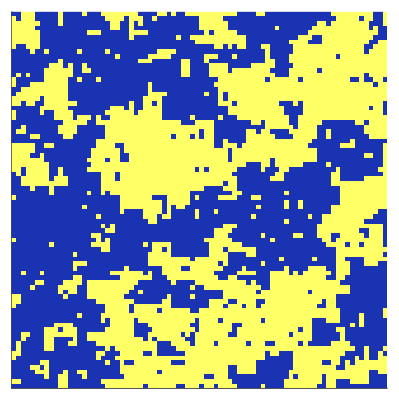
\includegraphics[width=100px, height=100px]{../data/snaps/snap80_temp2.26_moment100.png}
    \caption{MCS=100}
    \label{fig:image3}
  \end{subfigure}

  \caption{Siatka $80$x$80$, $T=2.26$}
  \label{fig:series}
\end{figure}

\begin{figure}[H]
  \centering

  \begin{subfigure}[b]{0.3\linewidth}
    \centering
    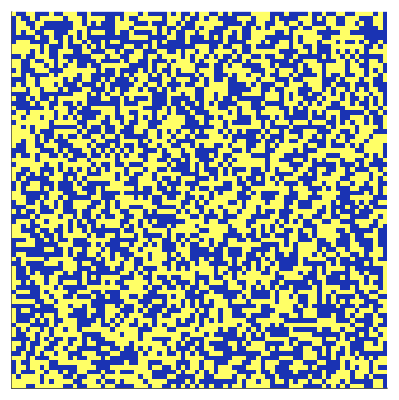
\includegraphics[width=100px, height=100px]{../data/snaps/snap80_temp4.0_moment1.png}
    \caption{MCS=0}
    \label{fig:image1}
  \end{subfigure}
  \hfill
  \begin{subfigure}[b]{0.3\linewidth}
    \centering
    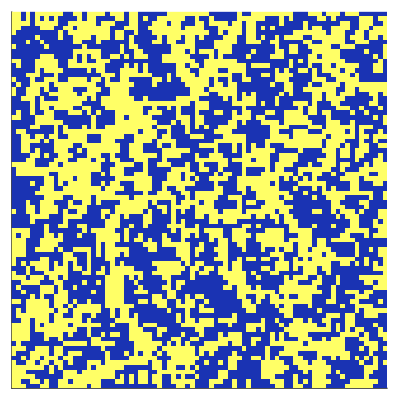
\includegraphics[width=100px, height=100px]{../data/snaps/snap80_temp4.0_moment50.png}
    \caption{MCS=50}
    \label{fig:image2}
  \end{subfigure}
  \hfill
  \begin{subfigure}[b]{0.3\linewidth}
    \centering
    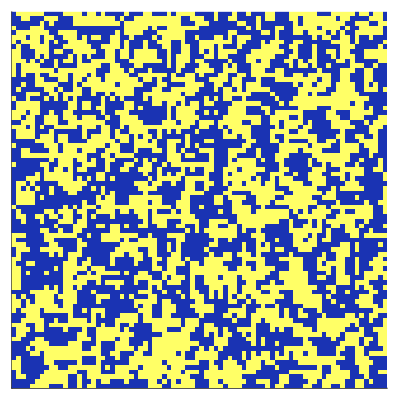
\includegraphics[width=100px, height=100px]{../data/snaps/snap80_temp4.0_moment100.png}
    \caption{MCS=100}
    \label{fig:image3}
  \end{subfigure}

  \caption{Siatka $80$x$80$, $T=4$}
  \label{fig:series}
\end{figure}


\subsection{Trajektorie magnetyzacji}

Na poniższych wykresach przedstawiono zmianę magnetyzacji układu w temperaturze $T=1$ dla różnych siatek. 

\begin{figure}[H]
  \centering

  \begin{subfigure}[b]{0.45\linewidth}
    \centering
	\centerline{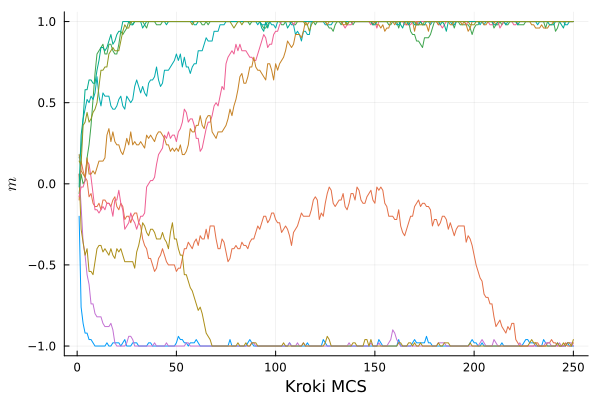
\includegraphics[scale=0.45]{../data/magnetizations/10.png}}
	\caption{$L=10$}
    \label{fig:image1}
  \end{subfigure}
  \hfill
  \begin{subfigure}[b]{0.45\linewidth}
    \centering
	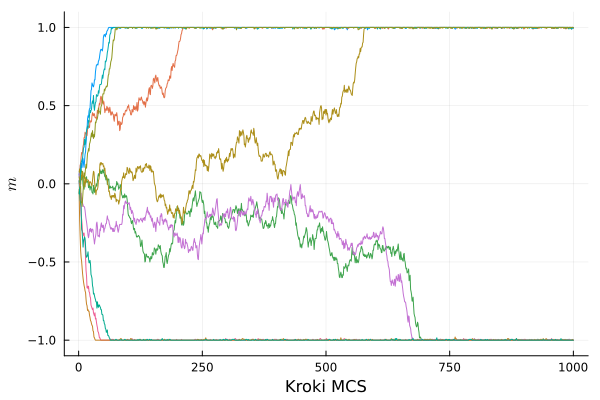
\includegraphics[scale=0.45]{../data/magnetizations/20.png}
	\caption{$L=20$}
    \label{fig:image2}
  \end{subfigure}

  \label{fig:series}
\end{figure}

\begin{figure}[H]
  \centering

  \begin{subfigure}[b]{0.45\linewidth}
    \centering
	\centerline{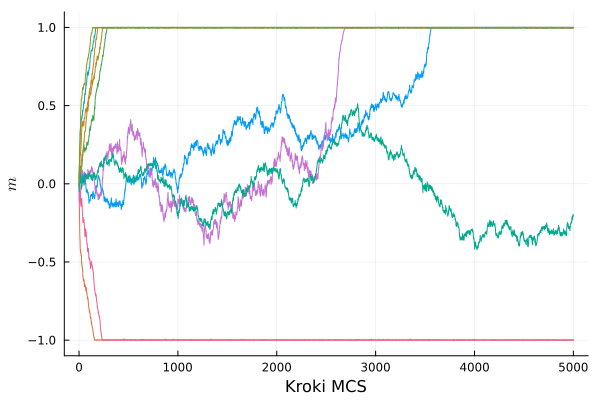
\includegraphics[scale=0.45]{../data/magnetizations/40.png}}
	\caption{$L=40$}
    \label{fig:image1}
  \end{subfigure}
  \hfill
  \begin{subfigure}[b]{0.45\linewidth}
    \centering
	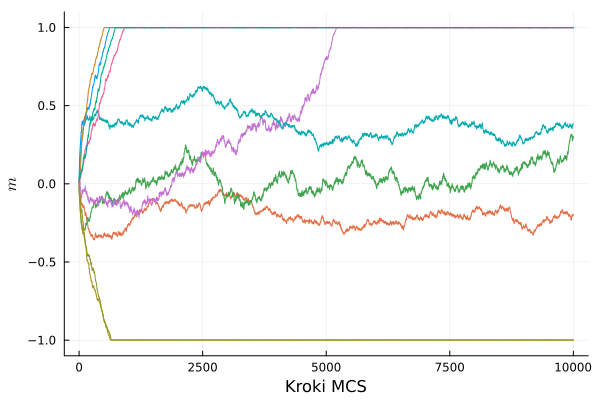
\includegraphics[scale=0.45]{../data/magnetizations/80.png}
	\caption{$L=80$}
    \label{fig:image2}
  \end{subfigure}

  \label{fig:series}
\end{figure}


\subsection{Trajektorie dla różnych temperatur}

Dla tych samych siatek przeprowadzono symulacje w 3 różnych temperaturach: poniżej krytycznej, krytycznej i powyżej. 


\begin{figure}[H]
  \centering

  \begin{subfigure}[b]{0.3\linewidth}
    \centering
    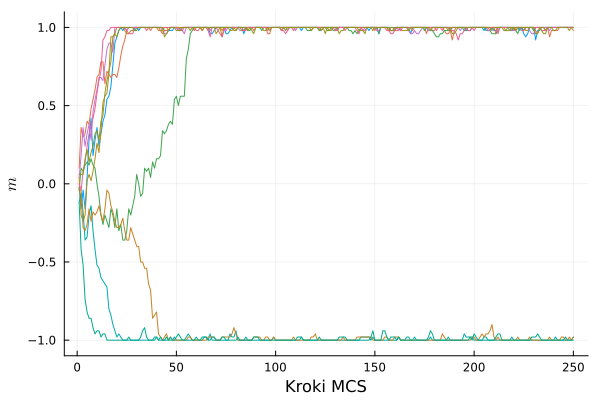
\includegraphics[width=150px, height=150px]{../data/magnetizations/10_T1.3.png}
    \caption{$T=1.3$}
    \label{fig:image1}
  \end{subfigure}
  \hfill
  \begin{subfigure}[b]{0.3\linewidth}
    \centering
    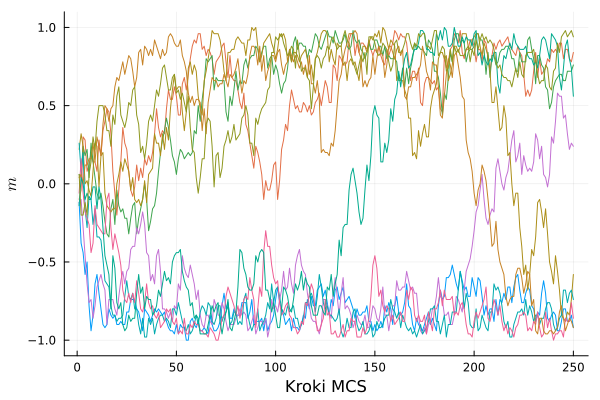
\includegraphics[width=150px, height=150px]{../data/magnetizations/10_T2.26.png}
    \caption{$T=2.26$}
    \label{fig:image2}
  \end{subfigure}
  \hfill
  \begin{subfigure}[b]{0.3\linewidth}
    \centering
    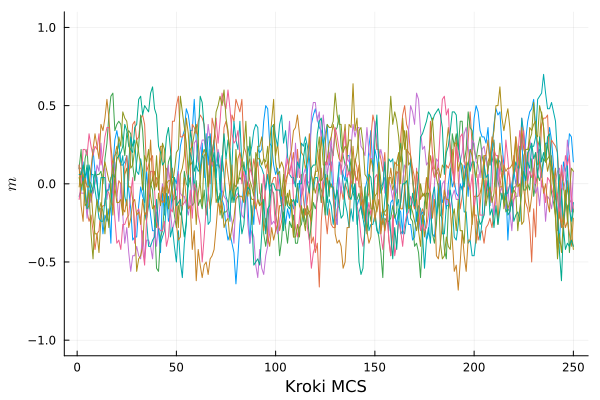
\includegraphics[width=150px, height=150px]{../data/magnetizations/10_T3.6.png}
    \caption{$T=3.6$}
    \label{fig:image3}
  \end{subfigure}

  \caption{$L=10$}
  \label{fig:series}
\end{figure}


\begin{figure}[H]
  \centering

  \begin{subfigure}[b]{0.3\linewidth}
    \centering
    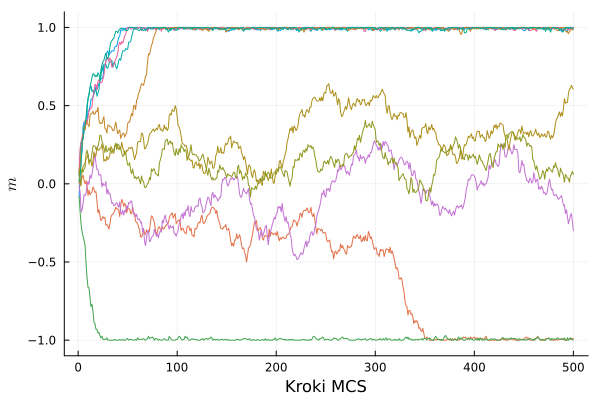
\includegraphics[width=150px, height=150px]{../data/magnetizations/20_T1.3.png}
    \caption{$T=1.3$}
    \label{fig:image1}
  \end{subfigure}
  \hfill
  \begin{subfigure}[b]{0.3\linewidth}
    \centering
    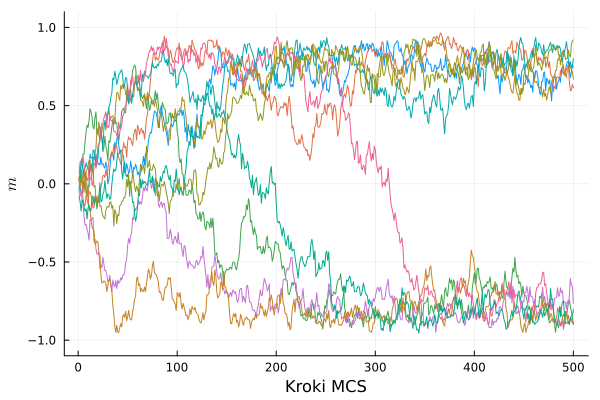
\includegraphics[width=150px, height=150px]{../data/magnetizations/20_T2.26.png}
    \caption{$T=2.26$}
    \label{fig:image2}
  \end{subfigure}
  \hfill
  \begin{subfigure}[b]{0.3\linewidth}
    \centering
    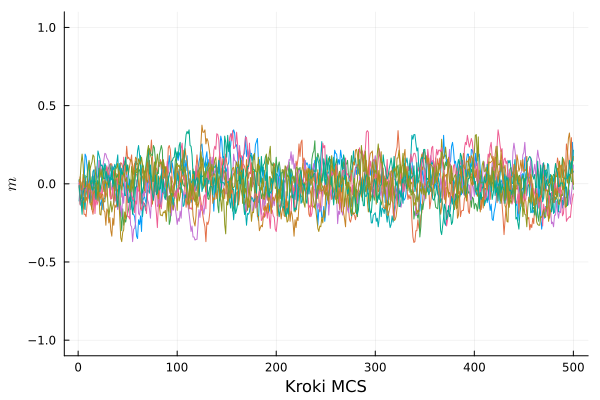
\includegraphics[width=150px, height=150px]{../data/magnetizations/20_T3.6.png}
    \caption{$T=3.6$}
    \label{fig:image3}
  \end{subfigure}

  \caption{$L=20$}
  \label{fig:series}
\end{figure}


\begin{figure}[H]
  \centering

  \begin{subfigure}[b]{0.3\linewidth}
    \centering
    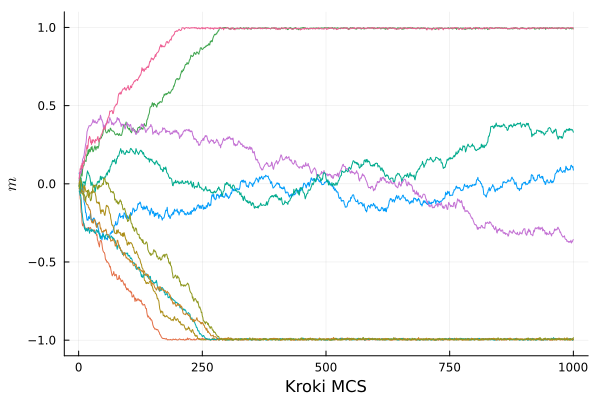
\includegraphics[width=150px, height=150px]{../data/magnetizations/40_T1.3.png}
    \caption{$T=1.3$}
    \label{fig:image1}
  \end{subfigure}
  \hfill
  \begin{subfigure}[b]{0.3\linewidth}
    \centering
    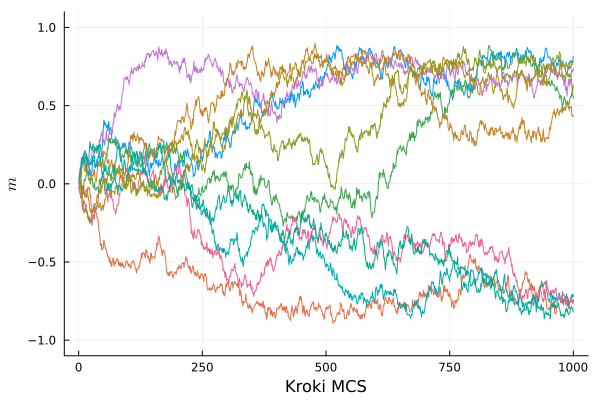
\includegraphics[width=150px, height=150px]{../data/magnetizations/40_T2.26.png}
    \caption{$T=2.26$}
    \label{fig:image2}
  \end{subfigure}
  \hfill
  \begin{subfigure}[b]{0.3\linewidth}
    \centering
    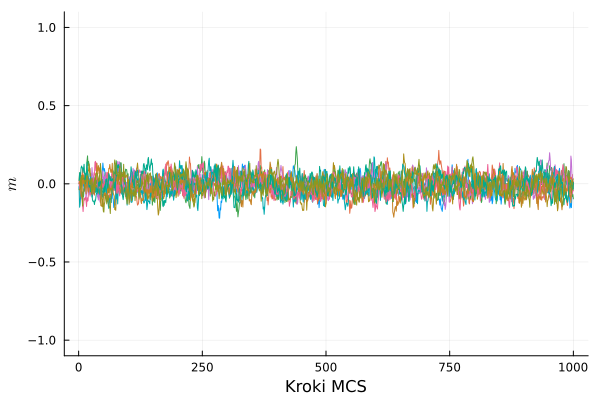
\includegraphics[width=150px, height=150px]{../data/magnetizations/40_T3.6.png}
    \caption{$T=3.6$}
    \label{fig:image3}
  \end{subfigure}

  \caption{$L=40$}
  \label{fig:series}
\end{figure}


\begin{figure}[H]
  \centering

  \begin{subfigure}[b]{0.3\linewidth}
    \centering
    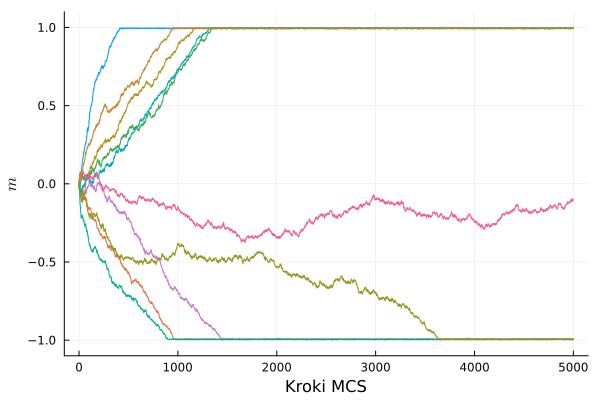
\includegraphics[width=150px, height=150px]{../data/magnetizations/80_T1.3.png}
    \caption{$T=1.3$}
    \label{fig:image1}
  \end{subfigure}
  \hfill
  \begin{subfigure}[b]{0.3\linewidth}
    \centering
    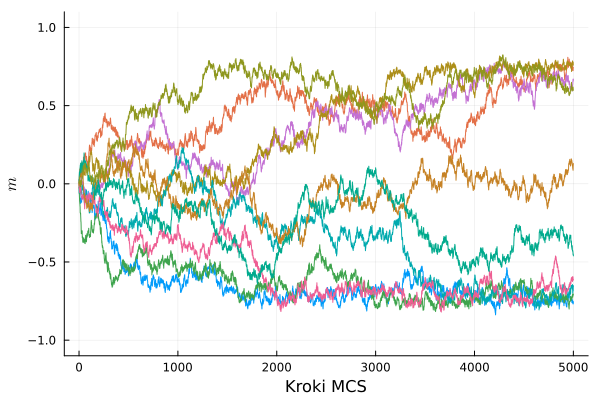
\includegraphics[width=150px, height=150px]{../data/magnetizations/80_T2.26.png}
    \caption{$T=2.26$}
    \label{fig:image2}
  \end{subfigure}
  \hfill
  \begin{subfigure}[b]{0.3\linewidth}
    \centering
    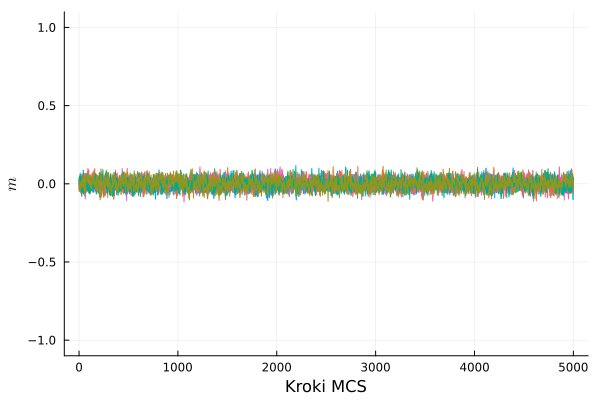
\includegraphics[width=150px, height=150px]{../data/magnetizations/80_T3.6.png}
    \caption{$T=3.6$}
    \label{fig:image3}
  \end{subfigure}

  \caption{$L=80$}
  \label{fig:series}
\end{figure}

\subsection{Magnetyzacja jako funkcja temperatury}

Poniżej znajdują się wykresy przedstawiające średnią magnetyzacje siatki w zależności od temperatury zredukowanej. Wykonano symulacje dla uśrednień po zespole jak i po czasie. 

\begin{figure}[H]
\centering
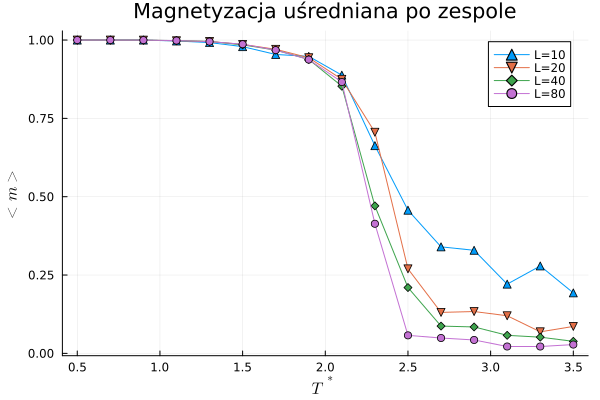
\includegraphics[scale=0.6]{../data/magnetizations/mag_temp.png}
\caption{$T^* \in (0,5; 3,5)\quad L \in \{10, 20, 40, 80\}$. Uśredniono po 30 zespołach}
\end{figure} 


\begin{figure}[H]
\centering
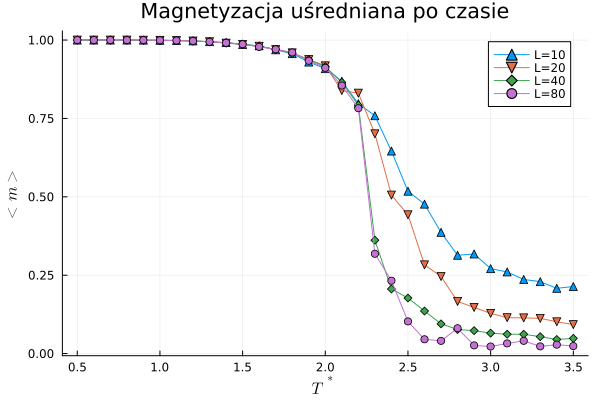
\includegraphics[scale=0.6]{../data/magnetizations/mag_time.png}
\caption{$T^* \in (0,5; 3,5)\quad L \in \{10, 20, 40, 80\}$. Uśredniono po czasie}
\end{figure} 


\end{document}